% !TeX root = document-en.tex

\chapter{Electric properties}
\label{chap:elec}

The framework for the electric properties, diffusion, mobility and einstein ratio will be detailed in this section. As now on, we will adopt the following formalism. If not stated otherwise, every quantity written in lowercase will be reduced and all the quantity in uppercase will be the non-reduced equivalent ($u_F$ is the reduced quantity of $U_F$). To reduce the unit we will use respectively for the energetic dimension and spatial dimension:

\begin{equation}
    \begin{aligned}
        u &= \frac{U}{k_bT}\\
        r &= 2\alpha R
    \end{aligned}
\end{equation}

$k_B$ being the Boltzmann constant and $\alpha = \SI{4.34e7}{cm^{-1}}$ the decay constant of the assumed hydrogen-like localized state wave functions.

\section{Gaussian formalism}

To simulate the localized behavior of charge carrier, we will use a gaussian density of states (gaussian DOS) for doped semiconductor. The doping effect will take form of an another gaussian with a different peak. The origin of the energy will be taken to be the LUMO level, but this theory works for holes and electron alike: an energy inversion is will bring us into the hole formalism.

\begin{equation}
    \begin{aligned}
    g\left(E, \hbar \omega_{\alpha}\right)=& \frac{1}{\sqrt{2 \pi}}\left\{\frac{N_{i-e}}{\sigma_{i}} \exp \left(-\frac{\left(E-\hbar \omega_{\alpha}\right)^{2}}{2 \sigma_{i}^{2}}\right)\right.\\
    &\left.+\frac{N_{d-e}}{\sigma_{d}} \exp \left(-\frac{\left(E-\hbar \omega_{\alpha}+E_{d}\right)^{2}}{2 \sigma_{d}^{2}}\right)\right\}
    \end{aligned}
    \label{eq:DOS_e}
\end{equation}

\begin{itemize}
    \item $N_{i-e}(cm^{-3})$: density of charge carriers for the intrinsic material
    \item $N_{d-e}(cm^{-3})$: density of charge carriers for the doped material
    \item $\hbar \omega_\alpha(J)$: mode effect, vibration of the lattice
    \item $\sigma_i(J)$: width of the intrinsic gaussian, representative of the disorder of the intrinsic material
    \item $\sigma_d(J)$: width of the doped gaussian, representative of the disorder of the doped material
    \item $E_D(J)$: energy shift between intrinsic and doped material
\end{itemize}

$g_e$ is expressed in $cm^{-3} J^{-1}$.

On the figure \ref{fig:3_2}, the doping results in a broadening of the DOS, which is coherent with doping increasing the number of states within the material.

\begin{figure}[htbp]
    \centering
    \begin{subfigure}[t]{0.49\textwidth}
        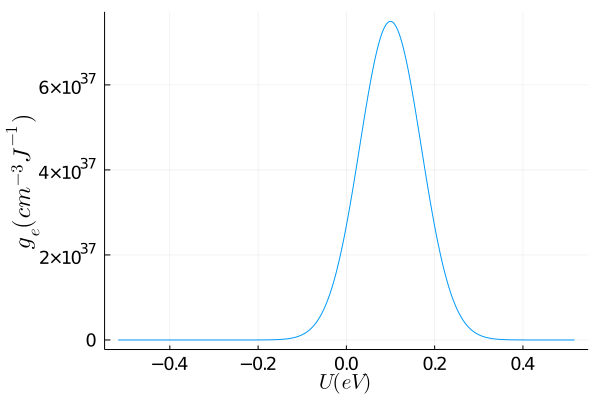
\includegraphics[width=\textwidth]{figures/3_elec/dos_undoped.png}
        \caption{Non-doped semiconductor}
    \end{subfigure}
    \begin{subfigure}[t]{0.49\textwidth}
        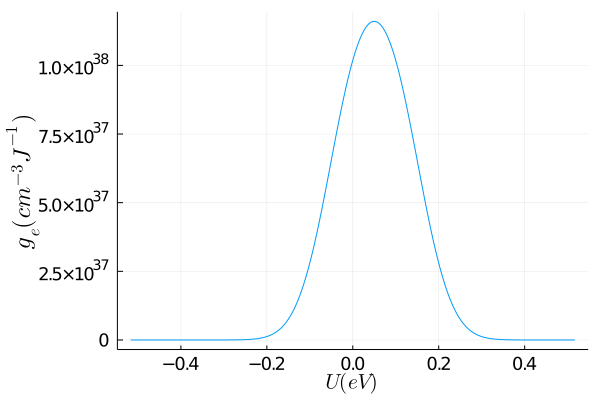
\includegraphics[width=\textwidth]{figures/3_elec/dos_doped.png}
        \caption{Doped semiconductor \\ $N_{d-e} = \SI{2.1e18}{cm^{-3}}$, $E_D = \SI{0.1}{eV}$}
    \end{subfigure}
    \caption[DOS]{DOS doping comparison \\ $T = 300K$, $N_{i-e} = \SI{2.1e18}{cm^{-3}}$, $\hbar \omega_\alpha = \SI{0.16e-19}{J}$}
    \label{fig:3_2}
\end{figure}

Using the Fermi-Dirac distribution, the carrier concentration is:

\begin{equation}
    n = \int_{-\infty}^{+\infty}\frac{g_e(U)}{1 + exp\left((\frac{U - (\hbar \omega_\alpha + U_F)}{k_BT}\right)}d U
\end{equation}

\section{Variable range hopping}

\subsection{Background}
We suppose that the charge carrier jump by tunneling from one state to another. The system is thus described in 4 dimensions: 3 for the spatial dimension, and one for the energy.

In our semi-classical model, we define the average probability for a jump to be the geometrical mean for all the jump within a material:

\begin{equation}
    \langle P \rangle = \operatorname{lim}_{n \rightarrow \infty}\left[\prod_{i}^{n} P_{i}\right]^{1 / n}=\exp \left[\operatorname{lim}_{n \rightarrow \infty} \frac{1}{n} \sum_{i}^{n} \ln P_{i}\right]
\end{equation}

$P_i$ being a singular jump in the material, we make the average over all the jump in the material.

As the arithmetic mean is more familiar, it's easier to work with the $\frac{1}{n} \sum_{i}^{n} \ln P_{i}$ part. To do so, we define the distance hopped to be:

\begin{equation}
    r_i = -ln(P_i)
\end{equation}

The $i$ arises from the fact that $P_i < 1$ and the logarithm is thus negative. Finally, we get:

\begin{equation}
    \langle P \rangle = exp(-r_{nn})
\end{equation}

With $r_{nn}$ being the mean range to the nearest neighbor for each state throughout the material. This theory making the average over all the states in the material has the advantage of summarizing the spatial and energy distribution of the states in on variable $r_{nn}$. The Miller-Abrahams hopping rate can now be written as:

\begin{equation}
    \nu = \nu_0 \cdot exp(-r_{nn})
    \label{eq:3_1.1}
\end{equation}

Usually, $\nu_0$ which is the basic hopping rate is set to $\SI{1e13}{Hz}$.

If we define $P_{ij}$ to be the probability of a jump from the state $i$ to the state $j$, from an energetic standpoint:

\begin{equation}
    P_{ij}^{energy} = exp\left(\frac{U_i - U_j}{k_BT}\right) = exp(u_i - u_j)
\end{equation}

From a spatial standpoint:

\begin{equation}
    P_{ij}^{spatial} = exp\left(-2\alpha L_{ij}\right) = exp(-l_{ij})
\end{equation}

We can fairly assume that:
\begin{equation}
    P_{ij} = P_{ij}^{total} = P_{ij}^{energy} \cdot P_{ij}^{spatial} = e^{[u_i - u_j] - l_{ij}} = e^{r_{ij}}
    \label{eq:3_1}
\end{equation}

We write the field effect as: $\beta = \frac{Fe}{2\alpha k_BT}$, $F$ being the field intensity in $V cm^{-1}$. Of course, the course of a charge carrier is modified by the field. To model this, we include it directly in the equation of the 4D distance: a state alongside the field direction will be seen as  closer or father depending on the angle $\theta$ between $R_{ij}$ and $F$:

\begin{equation}
    \left.\begin{array}{rlr}
    R_{i j} & =(1+\beta \cos \theta) L_{i j}+\left(U_{j}-U_{i}\right) & \text { for } U_{j}>U_{i}-\beta \cos \theta R_{i j} \\
    & =L_{i j} & \text { for } U_{j}<U_{i}-\beta \cos \theta R_{i j}
    \end{array}\right\}
    \label{eq:3_2}
\end{equation}

$(1+\beta \cos \theta)$ arises from the shift of the fermi level due to the field (fig. \ref{fig:R_max}). We assume here that for states to lower energy, only the physical distance is taken into account as the charge carrier does not need to make a jump to higher energies.

\subsection{Nearest neighbor}

The quantity $r_{nn}$ can be computed thanks to the formula of the "number of free states" $\mathscr{N}$, the mean number of free state at a distance $\mathscr{R}$ \footnote{Please note that the quantity $\mathscr{R}$ is reduced.} of a state. We suppose that the material is disorganized enough to make both energetic and spatial dimension uncorrelated, and that the states are equally distributed in respect of the gaussian DOS.

\begin{equation}
    \begin{aligned}
    \mathcal{N}\left(u, T, \beta, \mathscr{R}\right)=\int_{0}^{\pi} \int_{0}^{\mathscr{R}} \int_{-\infty}^{\mathscr{R}+u-r(1+\beta \cos \theta)} g\left(v\right)\left[1-F\left(v\right)\right] \frac{k_B T}{8 \alpha^{3}} \\
    \times 2 \pi r^2 \sin \theta d v d r d \theta
    \end{aligned}
    \label{eq:3_3}
\end{equation}

\begin{figure}[!h]
    \centering
    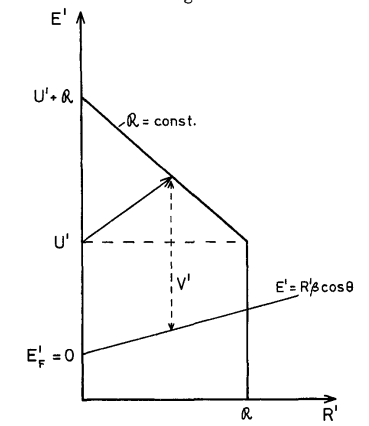
\includegraphics[width=.4\paperwidth]{figures/3_elec/R_max.png}
    \caption{Energetic-spatial relationship \label{fig:R_max} (source \cite{hopping_theory_1})}
\end{figure}

$g(1 - F)$ represent the emptiness of a state, $F$ being the Fermi-Dirac equation, $1 - F$ is the probability of the state to be empty, i.e a state where a charge carrier can jump. $\frac{k_B T}{8 \alpha^{3}}$ is simply a reducing factor to eliminate the unit of $g(1-F)$. $4\pi r^2$ is the surface of a sphere with a radius $r$ and $\frac{1}{2}\sin \theta$ makes the average between the field effect direction and the direction of $r$. The $\frac{1}{2}$ factor arises from the integral $\int_0^\pi \frac{1}{2}\sin \theta = 1$. The born in the energetic integral $\mathscr{R}+u-r(1+\beta \cos \theta)$ correspond to the maximum energetic value for a jump of distance $\mathscr{R}$. Finally, $\mathcal{N}$ computes the number of states enclosed enclosed in a 4D sphere of radius $\mathscr{R}$.

We thus define $r_{nn}$ being the radius at which we found in average, 1 free state, i.e $\mathcal{N}(r_{nn}) = 1$.

This method for computing $\mathscr{N}$ is similar to the percolation criteria, but they take $\mathcal{N}(r_{nn}) = 2.8$, $2.8$ being the percolation criteria. But, where the percolation theory intends to find a path of jump within the material, our $r_{nn}$ quantity means the nearest free states, which intuitively corresponds to the distance at which we find 1 state.

\begin{figure}[!h]
    \centering
    \includegraphics*[width=.5\paperwidth]{figures/3_elec/rnn.png}
    \caption{$r_{nn}$ behavior for pentacene, $F = \SI{5.3}{V . cm^{-1}}$ (pentacene parameters appendix \ref{pentacene})\label{fig:3_3}}
\end{figure}



From the figure \ref{fig:3_3}, we see that for low value of energy, the quantity $r_{nn}$ skyrockets. The rarefaction of available states due to the Fermi-Dirac distribution means that for a charge carrier to find an available spot is harder. On the opposite, we see a plateau at higher energetic values. At such energy, charge carrier can make energetically favorable jump to lower states, which depends only on the intrinsic characteristics of the material (the state distribution $g(1 - F)$). Mathematically, the born $\mathscr{R}+u-r(1+\beta \cos \theta)$ makes it happen: for lower $u$, $\mathscr{R}$ compensate to cover the spectrum $g(1 - F)$, and for higher energy, $u$ alone is enough to cover it.

\subsection{Real hopped distance}

With $r_{nn}$, we have an insight of the geometry of the material, but what really matters to find the diffusion or mobility is the average displacement of the charge carrier, that we will name $x_F$. Of course, such quantity is affected by the field intensity.

We first define:

\begin{equation}
    \begin{aligned}
    I_{1}&=\int_{0}^{\pi} \int_{u - r_{nn}\beta\cos \theta}^{u + r_{nn}} g(v)\left[1-F(v)\right]\left[\frac{r_{nn}-v+U^{\prime}}{1+\beta \cos \theta}\right]^{3} \sin \theta \cos \theta d v d \theta\\
    I_{2}&=\int_{0}^{\pi} \int_{-\infty}^{u - r_{nn}\beta\cos \theta} g(v)\left[1-F(v)\right] {r}_{n n}^{3} \sin \theta \cos \theta d v d \theta\\
    I_{3}&=\int_{0}^{\pi} \int_{u - r_{nn}\beta\cos \theta}^{u + r_{nn}} g(v)\left[1-F(v)\right]\left[\frac{r_{nn}-v+U^{\prime}}{1+\beta \cos \theta}\right]^{2} \sin \theta d v d \theta\\
    I_{4}&=\int_{0}^{\pi} \int_{-\infty}^{u - r_{nn}\beta\cos \theta} g(v)\left[1-F(v)\right] r_{nn}{ }^{2} \sin \theta d v d \theta
    \label{eq:3_I}
    \end{aligned}
\end{equation}

And the distance written as:

\begin{equation}
    x_F = \frac{I_1 + I_2}{I_3 + I_4}
    \label{eq:3_4}
\end{equation}

The eq. \ref{eq:3_4} is a weighted mean. $I_1$ and $I_3$ represent jumps to state of higher energy, thus involving not only the distance but the energy. $I_2$ and $I_4$ represent jumps to state of lower energy, thus involving only the spatial distance hopped.

$\left[\frac{r_{nn}-v+U^{\prime}}{1+\beta \cos \theta}\right]$ is comparable to a distance. If we take the expression $v = r_{nn}+u-r(1+\beta \cos \theta)$ from the eq. \ref{eq:3_3}, we find for the distance $r$:

\begin{equation}
    r = \left[\frac{r_{nn}-v+U^{\prime}}{1+\beta \cos \theta}\right]
\end{equation}

Moreover, to understand better the role of this integral, it is better to split it in two parts. First:

\begin{equation}
    w = g(v)\left[1-F(v)\right]\left[\frac{r_{nn}-v+U^{\prime}}{1+\beta \cos \theta}\right]^{2} \sin \theta d v
\end{equation}

This is the weight and represent the number of state at a certain distance $r$.

The function $f(v) = \left[\frac{r_{nn}-v+U^{\prime}}{1+\beta \cos \theta}\right] \cos \theta$ represents the distance to a free state pondered by the field effect $\cos \theta$.

Finally, we can sum up the relation \ref{eq:3_4} by:

\begin{equation}
    x_F = \frac{\int_{V_1} f(v)w(v) + \int_{V_2} f(v)w(v)}{\int_{V_1} w(v) + \int_{V_2} w(v)}
\end{equation}

With $V_1$ and $V_2$ being the surface of integration.

\begin{figure}[!h]
    \centering
    \includegraphics*[width=.5\paperwidth]{figures/3_elec/xf.png}
    \caption{$x_F$ dependence on energy, $F = \SI{5.3}{V . cm^{-1}}$ (pentacene parameters appendix \ref{pentacene})\label{fig:3_4}}
\end{figure}

The energy dependency (fig. \ref{fig:3_4}) see two plateaus, one a high energy is $0$, meaning that at this level, most of the jump are made only downward in energy. For the negative energies, the depletion in free state due to the Fermi-Dirac distribution makes the jump to be of a higher distance. But it reaches a plateau because at a certain point, the jump is made in energy to reach near Fermi level states.

\begin{figure}[!h]
    \centering
    \includegraphics*[width=.5\paperwidth]{figures/3_elec/I1.png}
    \caption{$I_1$ dependence on energy, $F = \SI{5.3}{V . cm^{-1}}$ (pentacene parameters appendix \ref{pentacene})\label{fig:3_5}}
\end{figure}


\begin{figure}[!h]
    \centering
    \includegraphics*[width=.5\paperwidth]{figures/3_elec/I2.png}
    \caption{$I_2$ dependence on energy, $F = \SI{5.3}{V . cm^{-1}}$ (pentacene parameters appendix \ref{pentacene})\label{fig:3_6}}
\end{figure}

By looking a little bit more into detail on $I_1$ and $I_2$ (fig. \ref{fig:3_5}, \ref{fig:3_5}), we can justify mathematically the global behavior of $x_F$. $I_2$ is similar to a gaussian bell because $g(1-F)$ dominates the integral. However, for $I_1$, for positive values we have indeed the lower born of the integral that $u - r_{nn}\beta \cos \theta$ that goes beyond the high density zone of states. Concerning the lower values, the increase of $r_{nn}$ compensate the decrease of energy $u$, making the upper limit $u + rnn$ more or less constant.

\begin{figure}[!h]
    \centering
    \includegraphics*[width=.5\paperwidth]{figures/3_elec/field_xf.png}
    \caption{$x_f$ dependence on the field, $F = \SI{5.3}{V . cm^{-1}}$ (pentacene parameters appendix \ref{pentacene})\label{fig:3_7}}
\end{figure}

By studying the influence of the field on $x_F$ (fig. \ref{fig:3_7}), we see that it reaches a limit at which $x_F$ decreases. Physically, the field increases so much that it starts extracting the charge carrier from the material. In top of that, $\lim_{x\to 0} xf = 0$. Indeed, if the charge carrier is not influenced by an electric field, its surrounding his uniform regarding the angle $\theta$, thus the jump are equidistant regarding all the direction.

\subsection{Mobility}

Mobility is classically defined as the average velocity of the particle divided by the force. In our case, the mean distance jumped being $x_F$ and a particle jumps at a rate (eq. \ref{eq:3_1.1}):

\begin{equation}
    \mu = \frac{\langle x \rangle}{F} = \dfrac{\nu_0 X_F e^{-r_{nn}}}{F}
    \label{eq:3_5}
\end{equation}

From the equation \ref{eq:3_5}, we can plot the mobility depending on the energy (figure \ref{fig:3_8}). At low energy, the charge carrier are globally trapped and can't participate to the mobility. However, at higher energy, we already noticed that the jump are made in great majority regarding the energy and not regarding spatial coordinates. Thus the mobility for higher value drops to $0$.

\begin{figure}[!h]
    \centering
    \includegraphics*[width=.5\paperwidth]{figures/3_elec/mobi_energy.png}
    \caption{$\mu$ dependence on the energy, $F = \SI{5.3}{V . cm^{-1}}$ (pentacene parameters appendix \ref{pentacene})\label{fig:3_8}}
\end{figure}

From the formula \ref{eq:3_5}, we can compute the conductivity $\sigma$:

\begin{equation}
    \sigma(U) = qg_e(U)F(U)\mu(U)k_B T
\end{equation}

We see on the figure \ref{fig:3_9} that the curve is shifted toward LUMO level. The majority of the free charge carrier being situated near this level, it is natural for the conductivity to do the same.

\begin{figure}[!h]
    \centering
    \includegraphics*[width=.5\paperwidth]{figures/3_elec/conduction_u.png}
    \caption{$\sigma$ dependence on the energy, $F = \SI{5.3}{V . cm^{-1}}$ (pentacene parameters appendix \ref{pentacene})\label{fig:3_9}}
\end{figure}


Of course the mobility is only defined for a sample affected by a field.

We define the global mobility in the material as $\mu(u)$ weighted by the number of states:

\begin{equation}
    \mu = \frac{\int_{-\infty}^{+\infty}\mu(u)g(u)F(u)du}{\int_{-\infty}^{+\infty}g(u)F(u)du}
\end{equation}

In a similar way, we define:

\begin{equation}
    \sigma = \frac{\int_{-\infty}^{+\infty}\sigma(u)g(u)F(u)du}{\int_{-\infty}^{+\infty}g(u)F(u)du}
\end{equation}

\subsection{Stochastic release time}

Stochastic release time, i.e the the transport time, is an essential concept for the diffusion. For higher $t$, we will have higher displacement and higher diffusion. The equation is similar to $x_f$ (eq. \ref{eq:3_4}):

\begin{equation}
    t = \frac{T_1 + T_2}{T_3 + T_4}
    \label{eq:t}
\end{equation}

We define $T_1$, $T_2$, $T_3$, $T_4$ as follow:

\begin{equation}
    \begin{aligned}
    T_{1}\left(u\right)=& \int_{0}^{\pi} d \theta \sin \theta \int_{0}^{r_{n n}} d r 2 \pi r^{2} \int_{u-r \beta \cos \theta}^{r_{n n}+u-r(1+\beta \cos \theta)} d \epsilon \\
    & \times \frac{g(u)(1 - F(v))}{v_{0}} \exp \left((1+\beta \cos \theta) r+\epsilon-u\right), \\
    T_{2}\left(u\right)=& \int_{0}^{\pi} d \theta \sin \theta \int_{0}^{r_{n n}} d r 2 \pi r^{2} \int_{-\infty}^{u-r \beta \cos \theta} d \epsilon \frac{g(u)(1 - F(v))}{v_{0}} \\
    & \times \exp ((1+\beta \cos \theta) r) \\
    T_{3}\left(u\right)=& \int_{0}^{\pi} d \theta \sin \theta \int_{0}^{r_{n n}} d r 2 \pi r^{2} \int_{u-r \beta \cos \theta}^{r_{n n}+u-r(1+\beta \cos \theta)} d \epsilon g(u)(1 - F(v)), \\
    T_{4}\left(u\right)=& \int_{0}^{\pi} d \theta \sin \theta \int_{0}^{r_{n n}} d r 2 \pi r^{2} \int_{-\infty}^{u-r \beta \cos \theta} d \epsilon g(u)(1 - F(v))
    \end{aligned}
\end{equation}

Similarly to eq.\ref{eq:3_I}, $g(1 - F)$ represents the emptiness of the arrival state. the exponential part can be summarized as: $exp(-r - u)$ and $\nu_0^{-1} exp(-r - u)$ represents the period of a jump. The born and the principle of the fraction is the same as for eq. \ref{eq:3_I}. Here again, $I_2$ differs from $I_1$ at it doesn't take into account the energy part: the jump is downward in energy and doesn't need any tunneling effect regarding the energy.

From the fig. \ref{fig:3_10}, we see that the time of a jump reaches $0$ for high value. From what has been previously deduced, at high energy the jumps (which are rare), occurs solely on the energy level, and thus are practically instantaneous. For lower value, the states being farther away with lower energy, the particle will obviously takes more time to jump.

\begin{figure}[!h]
    \centering
    \includegraphics*[width=.5\paperwidth]{figures/3_elec/time_u.png}
    \caption{$t$ dependence on the energy, $F = \SI{5.3}{V . cm^{-1}}$ (pentacene parameters appendix \ref{pentacene})\label{fig:3_10}}
\end{figure}

\subsection{Diffusivity}

From the definition of the diffusion, we have:

\begin{equation}
    D = \frac{1}{2 \cdot n} \frac{d}{d t} \langle x^2(t) \rangle
    \label{eq:3_6}
\end{equation}

\begin{itemize}
    \item $\langle x(t) \rangle$: average displacement of a particle
    \item $n = 3$: dimension of the system, in our case
\end{itemize}

However, in presence of an electric field, a drift term appears in the equation \ref{eq:3_6}:

\begin{equation}
    D = \frac{1}{2 \cdot n} \frac{d}{d t} \langle (X(t) - \langle X(t) \rangle)^2 \rangle
    \label{eq:3_7}
\end{equation}

$(X(t) - \langle X(t) \rangle$ is the drift of a certain displacement regarding the mean value. In a similar manner to eq. \ref{eq:3_5}, we get:

\begin{equation}
    \begin{aligned}
        D &= \frac{1}{2 \cdot n} \langle (X(t) - \langle X(t) \rangle)^2 \rangle \nu_0 e^{-r_{nn}} \\
        D &= \frac{1}{6} \langle X(t)^2 - 2X(t)\langle X(t) \rangle - \langle X(t) \rangle^2 \rangle \nu_0 e^{-r_{nn}} \\
        D &= \frac{1}{6} (\langle X(t)^2 \rangle - 2 \langle X(t)\rangle \langle X(t) \rangle - \langle X(t) \rangle^2) \nu_0 e^{-r_{nn}} \\
        D &= \frac{1}{6} (\langle X(t)^2 \rangle - \langle X(t) \rangle^2) \nu_0 e^{-r_{nn}} \\
    \end{aligned}
    \label{eq:3_8}
\end{equation}

We define $\Delta X$ as the average displacement around the average position $\langle X \rangle$ in a way that: $X = \langle X \rangle + \Delta X$. $\Delta X$ is the pure randomness rising from the charge displacement. If we substitute $X^2$ by this new relation in eq. \ref{eq:3_8}, we obtain:

\begin{equation}
    \begin{aligned}
        D &= \frac{1}{6} (\langle [\langle X \rangle + \Delta X]^2 \rangle - \langle X \rangle^2 \rangle) \nu_0 e^{-r_{nn}} \\
        D &= \frac{1}{6} (\langle \langle X \rangle^2 + 2\langle X \rangle\Delta X + \Delta X^2 \rangle - \langle X \rangle^2) \nu_0 e^{-r_{nn}} \\
        D &= \frac{1}{6} (2\langle X \rangle\Delta X + \Delta X^2 \rangle) \nu_0 e^{-r_{nn}} \\
    \end{aligned}
    \label{eq:3_9}
\end{equation}

We propose the following expression for $\Delta X$ and $\langle X \rangle$:

\begin{equation}
    \begin{aligned}
        \Delta X &= R_{nn} \\
        \langle X \rangle &= X_F t \nu_0 e^{-r_{nn}}
    \end{aligned}
    \label{eq:3_10}
\end{equation}

$\Delta X$ is thus the distance non-influenced by the field and $\langle X \rangle$ is being influenced both by the field (through $X_F$) and by the time of transport. The quantity $t \nu_0 e^{-r_{nn}}$ model the number of jump made by a charge carrier.

At the end, we obtain the following formula:

\begin{equation}
    D = \frac{1}{6} (2X_F t \nu_0 e^{-r_{nn}} + R_{nn}^2) \nu_0 e^{-r_{nn}}
    \label{eq:3_11}
\end{equation}

\begin{figure}[!h]
    \centering
    \includegraphics*[width=.5\paperwidth]{figures/3_elec/d_u.png}
    \caption{$D$ dependence on the energy, $F = \SI{5.3}{V . cm^{-1}}$ (pentacene parameters appendix \ref{pentacene})\label{fig:3_11}}
\end{figure}

From the figure \ref{fig:3_11}, we see that for higher energy levels, $D$ is higher. It is consistent with the precedent theory as with higher energy, particles have way more possibility to move. In \ref{eq:3_11}, we introduced $\Delta X$ which is the average deviation from the displacement and gives the constant value for higher energy as $r_{nn}$ also takes into account the energy part of the jumps.

In the same fashion as with the mobility, the diffusivity is defined throughout the material by:

\begin{equation}
    D = \frac{\int_{-\infty}^{+\infty}D(u)g(u)F(u)du}{\int_{-\infty}^{+\infty}g(u)F(u)du}
    \label{eq:3_12}
\end{equation}

\subsection{Einstein ratio}

From the precedent value we computed, we can now define the einstein ratio as we will use it. Fist, the energy dependent one writes as:

\begin{equation}
    EinsteinRatio(u) = \frac{D(u)}{\mu(u)}
    \label{eq:3_13}
\end{equation}

However, as the relation is usually referred to its original equation (eq. \ref{eq:2}), we will define $\eta$ as:

\begin{equation}
    \eta(u) = \frac{D(u)}{\mu(u)} \frac{q}{k_BT}
    \label{eq:3_14}
\end{equation}

\begin{figure}[!h]
    \centering
    \includegraphics*[width=.5\paperwidth]{figures/3_elec/ein_u.png}
    \caption{$\eta$ dependence on the energy, $F = \SI{5.3}{V . cm^{-1}}$ (pentacene parameters appendix \ref{pentacene})\label{fig:3_12}}
\end{figure}


From the figure \ref{fig:3_12}, we see that the einstein ratio attains a minimum for energy around the LUMO level. The value quickly rises for lower and higher energy level. For lower energy, it is admitted that traps cause higher $\eta$ value. For greater energies, the quick decrease of the mobility due to the lack of spatial displacement as well as the constant $D$ value due to the average variation of displacement $\Delta X$, helps $\eta$ ratio value to rise quickly.

\subsection{Summary of some numerical value}

To assess the viability of our model, we will perform some computation on the global values of $\mu$, $D$, and $\eta$.

We performed a computation with $F = \SI{4}{V cm^{-1}}$, to respect the value measured in Xavier's thesis \cite{xavier_thesis}.

\begin{center}
    \begin{tabular}{ |c||c|c|c|  }
        \hline
        & $\mu (\si{cm \cdot V^{-1} \cdot s^{-1}})$ & $D (\si{cm \cdot s^{-1}})$ & $\eta$ \\
        \hline
        \hline
        Values measured & $\SI{2.15e-5}{}$ & $\SI{2.85e-6}{}$ & $5.1$ \\
        \hline
        Simulation & $\SI{8.9e-5}{}$ & $\SI{5.45e-6}{}$ & $3.38$ \\
        \hline
    \end{tabular}
\end{center}

The order of magnitude for the simulated values are comparable. However, the final simulated value $\eta$ is a bit low compared to the real one measured. The overall mobility simulated is too high compared to the real one. It's due to a under-evaluated deep traps presence in the gaussian DOS. We also considered only energetic traps and spatial trap could be considered to reduce the overall mobility.

\section{Parameters influence}

Now that we have introduced all the parameters and equation for the electric part in our model, we can start to study the effect of different parameters on it.

\subsection{Electric Field}

The more obvious parameter to tweak is the field. It can easily be tuned by the bias voltage in a transistor for example.

\begin{figure}[!h]
    \centering
    \includegraphics*[width=.5\paperwidth]{figures/3_elec/d_field_low.png}
    \caption{$D$ dependence on low field (pentacene parameters appendix \ref{pentacene})\label{fig:3_13}}
\end{figure}

\begin{figure}[!h]
    \centering
    \includegraphics*[width=.5\paperwidth]{figures/3_elec/mobi_field_low_square.png}
    \caption{$\mu$ dependence on low field (pentacene parameters appendix \ref{pentacene})\label{fig:3_14}}
\end{figure}

\begin{figure}[!h]
    \centering
    \includegraphics*[width=.5\paperwidth]{figures/3_elec/ein_field_low.png}
    \caption{$\eta$ dependence on low field (pentacene parameters appendix \ref{pentacene})\label{fig:3_15}}
\end{figure}

For lower field ($\sim \SI{1e4}{V \cdot cm^{-1}}$), we observe a linearity for $D$ (fig. \ref{fig:3_13}). Regarding the mobility, we clearly see a quadratic dependence on the field (fig. \ref{fig:3_14}). However, if we look closer at the numerical value, we can notice that for lower field the mobility is more or less constant. At the end, thanks to a constant mobility and a linear diffusivity regarding the field, the $\eta$ value is also constant.

By increasing the field ($\sim \SI{1e5}{V \cdot cm^{-1}}$), we can observe a new behavior for the electric characteristics (fig. \ref{fig:3_16}, \ref{fig:3_17}, \ref{fig:3_18}).

\begin{figure}[!h]
    \centering
    \includegraphics*[width=.5\paperwidth]{figures/3_elec/d_field_high_square.png}
    \caption{$D$ dependence on high field (pentacene parameters appendix \ref{pentacene})\label{fig:3_16}}
\end{figure}

\begin{figure}[!h]
    \centering
    \includegraphics*[width=.5\paperwidth]{figures/3_elec/mobi_field_high_square.png}
    \caption{$\mu$ dependence on high field (pentacene parameters appendix \ref{pentacene})\label{fig:3_17}}
\end{figure}

\begin{figure}[!h]
    \centering
    \includegraphics*[width=.5\paperwidth]{figures/3_elec/ein_field_high.png}
    \caption{$\eta$ dependence on high field (pentacene parameters appendix \ref{pentacene})\label{fig:3_18}}
\end{figure}

Indeed, the diffusivity $D$ starts having quadratic behavior, as described in the paper \cite{general_einstein}. While the mobility still has a quadratic behavior (fig. \ref{fig:3_17}), it seems that the increase is greater for the $\mu$ value and that the einstein ratio $\eta$ sees a local maximum for higher field (fig. \ref{fig:3_18}).

\subsection{Temperature}